\documentclass[journal]{vgtc}                % final (journal style)
%\documentclass[review,journal]{vgtc}         % review (journal style)
%\documentclass[widereview]{vgtc}             % wide-spaced review
%\documentclass[preprint,journal]{vgtc}       % preprint (journal style)
%\documentclass[electronic,journal]{vgtc}     % electronic version, journal

%% Uncomment one of the lines above depending on where your paper is
%% in the conference process. ``review'' and ``widereview'' are for review
%% submission, ``preprint'' is for pre-publication, and the final version
%% doesn't use a specific qualifier. Further, ``electronic'' includes
%% hyperreferences for more convenient online viewing.

%% Please use one of the ``review'' options in combination with the
%% assigned online id (see below) ONLY if your paper uses a double blind
%% review process. Some conferences, like IEEE Vis and InfoVis, have NOT
%% in the past.

%% Please note that the use of figures other than the optional teaser is not permitted on the first page
%% of the journal version.  Figures should begin on the second page and be
%% in CMYK or Grey scale format, otherwise, colour shifting may occur
%% during the printing process.  Papers submitted with figures other than the optional teaser on the
%% first page will be refused.

%% These three lines bring in essential packages: ``mathptmx'' for Type 1
%% typefaces, ``graphicx'' for inclusion of EPS figures. and ``times''
%% for proper handling of the times font family.

\usepackage{mathptmx}
\usepackage{graphicx}
\usepackage{times}
\usepackage{epstopdf}
\usepackage{amsmath}
\usepackage{multirow} 
\usepackage{amsmath}
\usepackage{color}



%% We encourage the use of mathptmx for consistent usage of times font
%% throughout the proceedings. However, if you encounter conflicts
%% with other math-related packages, you may want to disable it.

%% This turns references into clickable hyperlinks.
\usepackage[bookmarks,backref=true,linkcolor=black]{hyperref} %,colorlinks
\hypersetup{
  pdfauthor = {},
  pdftitle = {},
  pdfsubject = {},
  pdfkeywords = {},
  colorlinks=true,
  linkcolor= black,
  citecolor= black,
  pageanchor=true,
  urlcolor = black,
  plainpages = false,
  linktocpage
}

%% If you are submitting a paper to a conference for review with a double
%% blind reviewing process, please replace the value ``0'' below with your
%% OnlineID. Otherwise, you may safely leave it at ``0''.
\onlineid{0}

%% declare the category of your paper, only shown in review mode
\vgtccategory{Research}

%% allow for this line if you want the electronic option to work properly
\vgtcinsertpkg

%% In preprint mode you may define your own headline.
%\preprinttext{To appear in IEEE Transactions on Visualization and Computer Graphics.}

%% Paper title.

\title{Real-Time Exploratory Visual Analysis Big Data }

%% This is how authors are specified in the journal style

%% indicate IEEE Member or Student Member in form indicated below
%\author{Roy G. Biv, Ed Grimley, \textit{Member, IEEE}, and Martha Stewart}
%\authorfooter{
%% insert punctuation at end of each item
%\item
% Roy G. Biv is with Starbucks Research. E-mail: roy.g.biv@aol.com.
%\item
% Ed Grimley is with Grimley Widgets, Inc.. E-mail: ed.grimley@aol.com.
%\item
% Martha Stewart is with Martha Stewart Enterprises at Microsoft
% Research. E-mail: martha.stewart@marthastewart.com.
%}

%other entries to be set up for journal
%\shortauthortitle{Biv \MakeLowercase{\textit{et al.}}: Global Illumination for Fun and Profit}
%\shortauthortitle{Firstauthor \MakeLowercase{\textit{et al.}}: Paper Title}

%% Abstract section.
\abstract{
Exploratory visual analysis is crucial  to making sense of increasingly large data sets, sometimes with millions or more records. Designing an exploratory big data visual analysis system for real time interaction is challenging. In this paper, we summarize the challenges to big data visual analysis systems from two aspects: 1) system architecture to support high performance and low latency for enabling real-time user interaction, and 2) interaction techniques to help analysts handle millions of items for quickly identifying a needle in a haystack. We propose our solution to exploratory big data analysis: AVIST -- a GPU based animated visualization toolkit targeting  big time-series, multi-dimensional data sets. Our first contribution is a GPU based in-situ visualization architecture for data processing/mining running simultaneously with visual rendering, which maximizes GPU parallel computing capability and reduces I/O costs for data transformation. To further improve the performance, we propose a data dependency graph design based on an incremental computing idea. We also employ user interaction techniques to trigger such incremental computation. Those interactions such as animation, associated data filters, brushing and linking can help analysts quickly get  insights from data. At last, we demonstrate that our system can easily identify abnormal behaviors and infer hypothesis in two case studies. 
} % end of abstract

%% Keywords that describe your work. Will show as 'Index Terms' in journal
%% please capitalize first letter and insert punctuation after last keyword
\keywords{Big data, interactive data exploration and discovery}

%% ACM Computing Classification System (CCS). 
%% See <http://www.acm.org/class/1998/> for details.
%% The ``\CCScat'' command takes four arguments.

\CCScatlist{ % not used in journal version
 \CCScat{K.6.1}{Management of Computing and Information Systems}%
{Project and People Management}{Life Cycle};
 \CCScat{K.7.m}{The Computing Profession}{Miscellaneous}{Ethics}
}

%% Uncomment below to include a teaser figure.
%   \teaser{
%   \centering
%   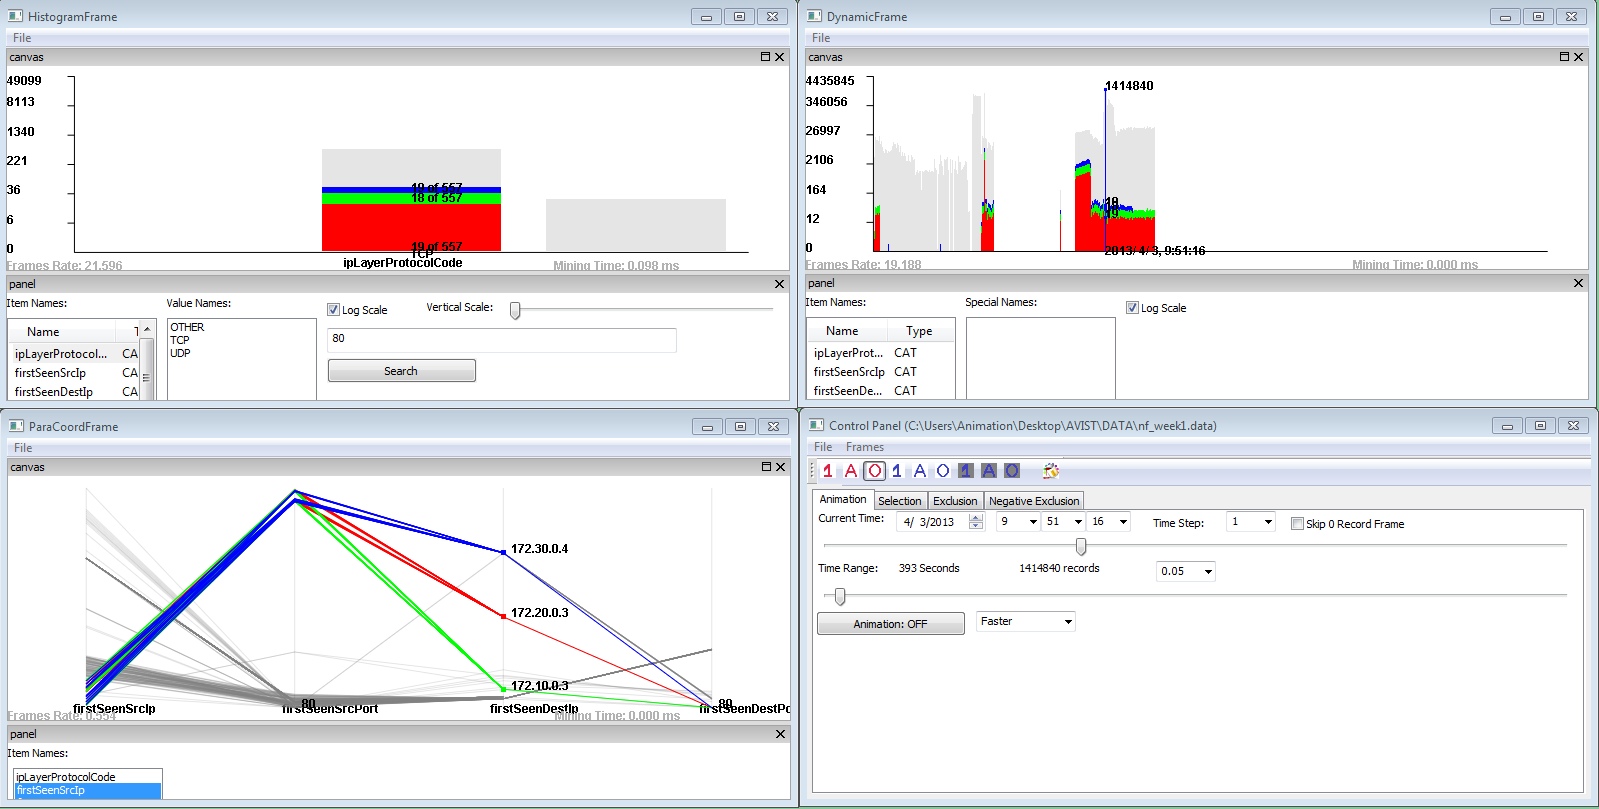
\includegraphics[width=16cm]{DataView.png}
   %	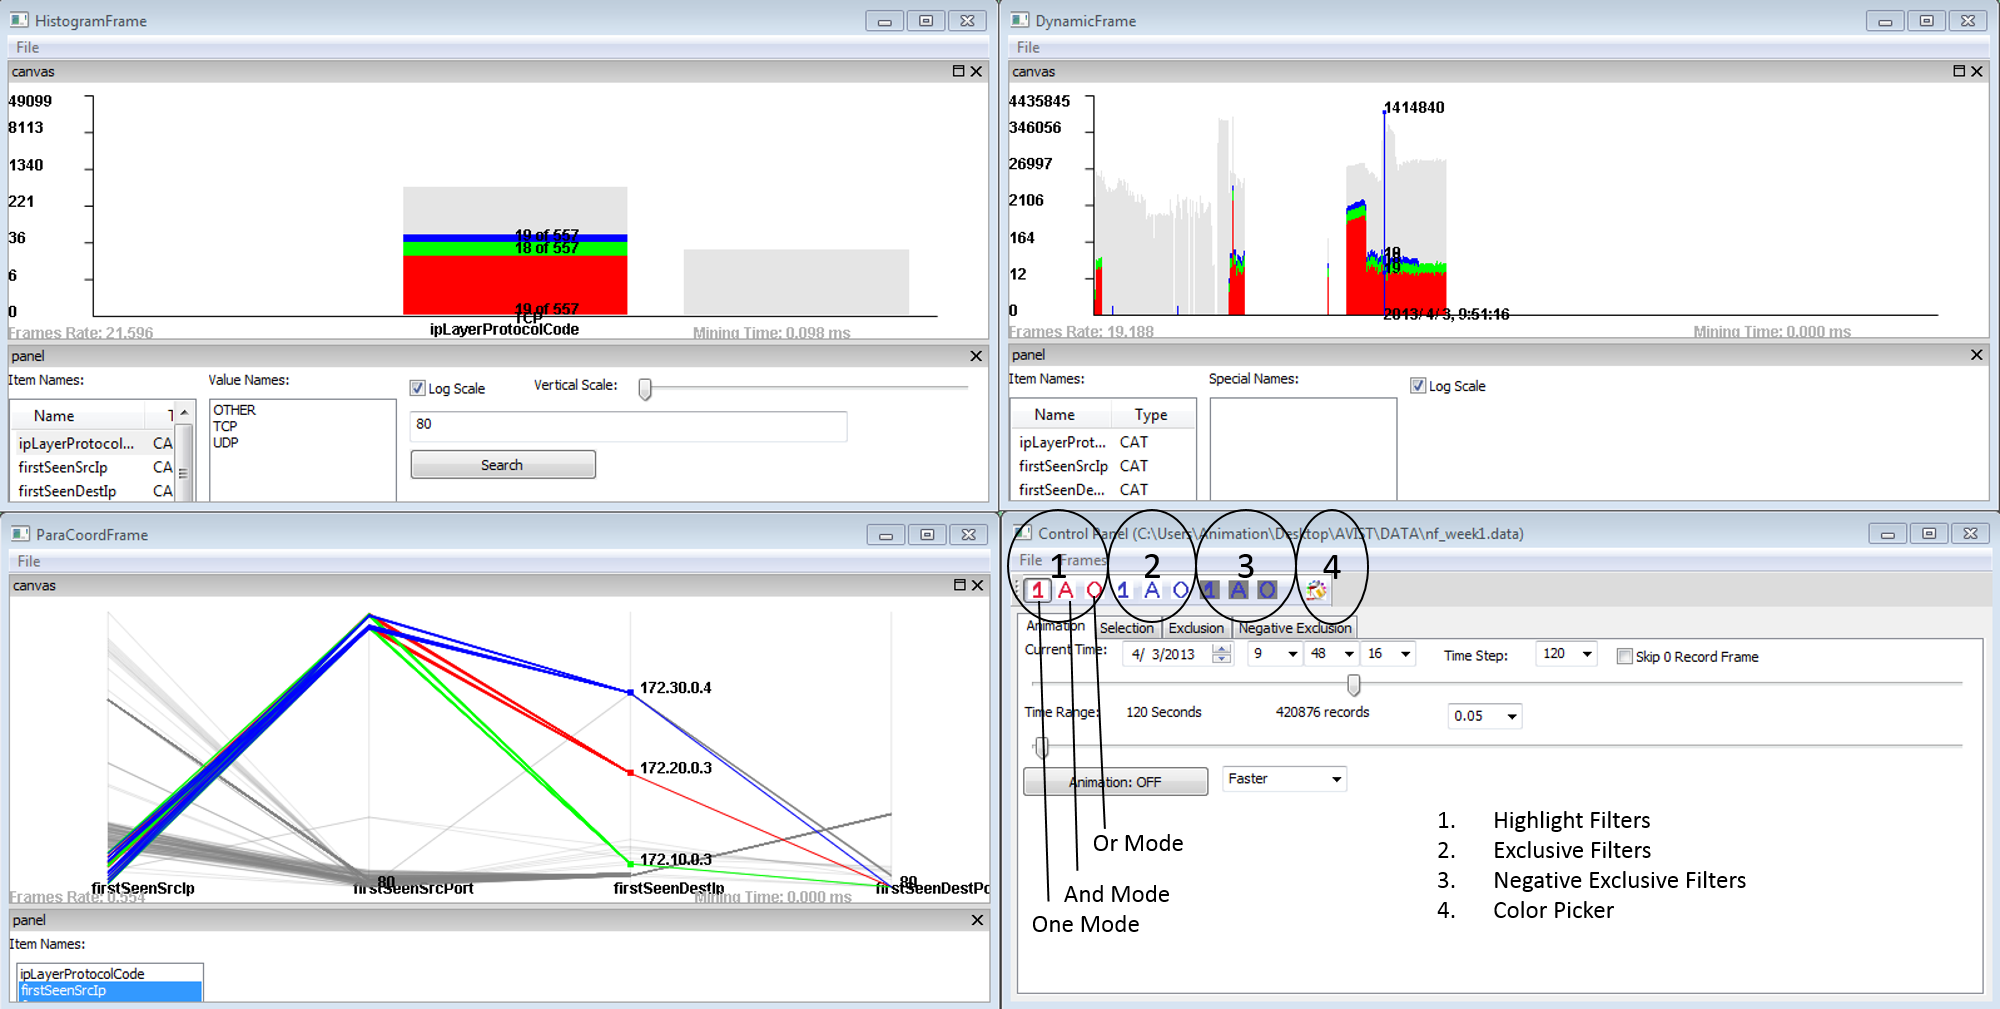
\includegraphics[width=1.0]{pic/DataView.png}
%   \caption{In the Clouds: Vancouver from Cypress Mountain.}
%  }

%% Uncomment below to disable the manuscript note
%\renewcommand{\manuscriptnotetxt}{}

%% Copyright space is enabled by default as required by guidelines.
%% It is disabled by the 'review' option or via the following command:
% \nocopyrightspace

%%%%%%%%%%%%%%%%%%%%%%%%%%%%%%%%%%%%%%%%%%%%%%%%%%%%%%%%%%%%%%%%
%%%%%%%%%%%%%%%%%%%%%% START OF THE PAPER %%%%%%%%%%%%%%%%%%%%%%
%%%%%%%%%%%%%%%%%%%%%%%%%%%%%%%%%%%%%%%%%%%%%%%%%%%%%%%%%%%%%%%%%

\begin{document}

%% The ``\maketitle'' command must be the first command after the
%% ``\begin{document}'' command. It prepares and prints the title block.

%% the only exception to this rule is the \firstsection command
\firstsection{Introduction}

\maketitle

%% \section{Introduction} %for journal use above \firstsection{..} instead
Visual analysis (VA) is "the science of analytical reasoning facilitated by interactive visual interfaces" \cite{Thomas2005} and visual analysis systems are crucial to supporting analysts for sense-making, reasoning and decision making. Previous visual analysis systems focus more on novel visualization and interaction techniques. As more and more data are generated at high volume and with increasing complexity, the solutions for scaling VA systems to big data require further investigation\cite{Zhang2012}. While the definition of "big data" is debatable, in this paper we follow an existing definition from previous research and use one million or more data items as a threshold \cite{2013-immens}.
     
Exploratory visual analysis is important for insight discovery in big data. When faced with big data, analysts may not realize what they do not know. Exploratory analysis is a way for "unknown-unknown" knowledge discovery: exploring the data, formulating possible hypotheses, and exploring the data again for verification or new hypotheses generation. In this paper, we focus on designing a VA system for exploratory analysis of big data. Specifically, we target the high volume of time-series and multi-dimensional data. We present AVIST: a GPU based animation visualization toolkit for real time visual exploration of such data. We hope that AVIST can potentially assist cyber security analysts  find potential threats from big router logs and help financial analysts to analyze custom transactions to provide better services.

Research about big data exploratory visual analysis systems should answer two key questions: 1) system design for handling big data to support real time interaction, and 2) interaction and visualization techniques to facilitate big data interpretation. The former question is related with the data processing techniques and database design. The latter concerns the scalability of visualizations and interactions. In this paper, we carefully consider these two questions and present AVIST for real time visual exploration of big data.

\textbf{GPU based In-Situ Visualization Architecture.} Previous research tackles the big data problem from the data reduction and compression aspects. While we admit their contributions for data sampling, aggregation, and modeling, we argue that the raw data is more important and attempt to prevent losing information during the data processing stage. This is important for exploratory data analysis. We aim at helping analysts to find a needle in haystack, rather than telling them the shape of the haystack or the distribution of the needles. In this paper, we provide a GPU based in-situ visualization architecture, which stores all raw data in GPU memory and  features the data processing and visual rendering simultaneous based on the powerful GPU parallel computing performance. 

\textbf{Big data visualization and interactions.} Visualizing millions of items in a given resolution of display ({$1{\sim}3$ million pixels) may have perceptual and interactive problems \cite{2013-immens}. We agree that visualizing all data points may lead to over-plotting and may overwhelm users' perceptual and cognitive capacities. However, mostly this problem happens due to lacking of efficient interaction techniques for exploring big data. We argue that visually presenting all data items and providing powerful user interactions for filtering large data can help users perceive more. For exploratory analysis, over-plotting may indicate some kind of information that users need to perceive and may direct users' attention to  next interactions and hypotheses . In AVIST system, we incorporate animation, combined data filters and brushing and linking interaction techniques to facilitate users to explore large data and enable them to find a needle in haystack. Besides, we carefully design the data flow in AVIST and present a data dependency graph to incorporate those interactions for incremental computing. 
	 
In this paper, we present the AVIST system for real-time exploratory visual analysis of big time-series and multidimensional datasets. The AVIST system features a GPU based in-situ visualization architecture that combines multiple visualizations and interaction techniques to help users drill down into big data in real-time. We use two cases to demonstrate the features of our system.
      



\section{Related Work}
Big data visual analysis systems are related to lots of research areas. In this section, we survey previous research from three aspects: 1) system design and data processing for real-time handling of big data, 2) visualization and interaction techniques that can scale to big data, and 3) parallel computing for big data visual analysis. 
 


\subsection{VA Systems and Data Processing }
Both academia and industry are interested in designing big data visualization systems and propose solutions from different aspects.

Companies have already released their VA systems for the growing market. \textit{Tableau} \cite{tab} is the pioneer and it can handle big data based on its Tableau Data Engine (TDE) \cite{Wesley}, which is a specialized column store modeled after MonetDB \cite{Boncz05monetdb}. \textit{QlikView} \cite{qlikview} is also a major player regarding in-memocry architecture to support interactive drill-down capabilities. \textit{Spotfire} \cite{spotfire} is awarded for its automatic analytics, interactive visualization, and system architecture and data management. Zhang et al. \cite{Zhang2012} survey the state-of-art commericial VA frameworks (e.g. \textit{Tableau} \cite{tab}, \textit{QlikView} \cite{qlikview}, \textit{Spotfire} \cite{spotfire}, \textit{JMP} \cite{jmp}, etc.), and point that there is still room for improvement and a number of challenges for future directions such as real time analysis, predictive analysis and so on.

Actually, lots of commercial products have roots in academic research such as \textit{Tableau} \cite{tab} from Stanford University and \textit{Spotfire} \cite{spotfire} from University of Maryland. Academic researchers are more active in big data visual analysis system. In the database community, research about in-memory databases and data cubes are the foundations of manipulating big data in VA systems for supporting real-time interaction. Recent big data visual analytics systems such as Nanocubes \cite{Lins2013} and imMens \cite{2013-immens} are based on the data cube idea. SAP designs Hana-DB \cite{farber2012sap} which is an in-memory database system for business analytical applications. Besides, data aggregation methods are also investigated. imMens \cite{2013-immens} emphasizes  binned aggregation. Jugel et al. \cite{jugel2014m4} propose a new visualization oriented data aggregation technique for visualizing big time-series data. Query performance is also an important issue for VA systems. Agarwal et al. \cite{Agarwal} propose BlinkDB which allows users to trade-off query accuracy for response time. Fisher et al. \cite{Fisher2012} also propose a similar idea about approximate database queries for exploratory data analysis. To further improve performance, the paper suggests to run queries on incremental samples to achieve real-time interaction. VisReduce \cite{im2013visreduce} provides incremental computing visualization and is based on a modified Map-Reduce-style algorithm. 


In the visual analytics field, researchers are more interested in the methodology of the visual analysis system. Fekete et al. \cite{Fekete2013} emphasize VA systems  on three important layers: visualization, analytics and data management. This paper analyzes the main issues of each layer to support interactive exploration of big data. Morton et al. \cite{morton2014support} present a vision of next-generation visual analytics services covered three related capabilities inspired by the sense-making model. Stolper et al. \cite{Stolper2014} give the progressive visual analytics model which enables an analyst to inspect partial results without sacrificing computing speed. Battle et al. \cite{battle2013dynamic} present a three-tiered visualization system for automatic reduction of the query results.
 


\subsection{Visualization and Interaction}
Visualization of big data often results in occlusion and cluttering problems.  Researchers in information visualization area have proposed many clutter reduction techniques. Ellis et al. \cite{Ellis2007} give a taxonomy of clutter reduction techniques which can be divided into three categories. 1) Appearance - the methods to affect the look of data items such as point size, opacity (alpha blending), sampling and filtering. 2) Spatial distortion includes topological distortion (fish-eye), pixel plotting, and dimensional reordering and spacing-filling techniques. 3) The last is animation technique. This paper argues that all of these cluttering reduction techniques match different problems where different criteria may have different importance. Besides, Fekete et al. \cite{Fekete:2002} propose several non-standard visual attributes such as stereovision or synthetic overlap count to enhance visualization. Chen et al. \cite{chen2014visual} give a hierarchical multi-class sampling techniques for feature preservation while reducing the total visual elements.

Another challenge for big data visualization is the human interaction techniques to facilitate users quickly identifying patterns and outliers. Fekete et al. \cite{Fekete:2002} summarize the interactive techniques from four aspects:
space multiplexing, time multiplexing, overlapping and space deformation. Space multiplexing is displaying two or more visualization configurations on the same screen while the time multiplexing technique shows each configuration successively at regular pace (animation) or by iterative methods such as dynamic queries. Over-plotting shows transient information over the visualization and space-deformation only shows important features based on sampling and aggregation. Cross filtering \cite{weaver2010cross} is also an important interaction technique for exploring big data with high dimensional attributes which supports expression of complex multidimensional queries using simple interactions. Polaris \cite{stolte2002polaris} is well known as generating a precise set of relational queries from the visual specifications,and such kind of ad hoc query mechanism is critical to exploratory data analysis for supporting users hypotheses generation and verification.



\subsection{Parallel Computing}
Parallel computing and distributed systems are becoming significant parts of big data visual analysis systems.  Google has designed Dremel \cite{melnik2010dremel}, a distributed system for interactive analysis of large scale nested data. Based on Hadoop, Starfish \cite{herodotou} is a self-tuning system for big data analytics. It adapts to user needs and workloads to provide better performance. Chen et al. \cite{Chen:2012} survey  Map-Reduce based systems for interactive query processing of big data and point to new design directions for shifting from long-running batch jobs to interactive analysis.

GPUs are designed for videogame and graphics but their remarkable development in performance and programmability makes them popular for general purpose computing and a number of researchers have proposed GPU based solutions for big data analysis. Fekete et al. \cite{Fekete:2002} emphasize using accelerated graphics hardware to provide high-density interactive visualization. imMens \cite{2013-immens} supports interactive visualization of big data based on parallel query processing. Zinsmaier et al. \cite{zinsmaier} utilize GPU computing for real time interaction with million node graphs.

\section{Design Analysis}
We emphasize real time visual exploration of big data. We argue that such VA systems need to support users \textbf{finding a needle in haystack}. VA systems should provide \textbf{real time drill down querying} of big data to help user find outliers and identify pattens. Based on these guidelines, we summarize and analyze previous techniques for designing VA systems.

\subsection{Data Processing}
First, we focus on database design and query processing. We want to achieve both high performance and support for ad hoc querying in our VA system.  
 
\textbf{In-memory database} is a popular technique in commercial big data VA products. Compared with traditional on-disk databases, in-memory databases are faster at accessing data by eliminating seek time, which guarantees faster and more predictable performance. While the memory capability constrains  data size, solutions such as hybrid database systems or distributed in-memory architectures \cite{Kallman:2008}  are next research directions.  

\textbf{Data cube} is an aggregate operator for On Line Analytical Processing (OLAP) in the context of data warehousing. However, cube size explodes as data dimensionality increases, which has a significant storage requirement even than original datasets. Besides, data cube needs heavily pre-computing for aggregation, and is hardly to support query down to any individual record.

\textbf{Approximated and incremental queries} are promising techniques for big data analysis. Fisher et al. \cite{FisherCHI2012} show the utility of the approximated queries by interviewing three teams of analysts,  and they conclude that incremental query interactions for data analysis is tractable and desirable. Analysts can obtain immediate feedback by incremental queries to refine their results, even further to explore new avenues.  

\textbf{Data reduction} are general methods for dealing with big data, including filtering, sampling, aggregation and modeling. Liu et al. \cite{2013-immens} give a survey about data reduction techniques. And this paper argues that sampling strategies and model based abstractions require prior knowledge and preprocessing of big data, while filtering and aggregation techniques are more effective in some cases. They adopt data aggregation technique to generate data cubes for real time visual query. However, this paper cannot afford ad hoc queries.   

In all, we summarize major techniques for designing the database and processing query in table\ref{tab:database}, which guide the design of our VA system. Because we aim to support ad hoc query and drill down interaction, data cube technique is not our choice. Data sampling and modeling need prior knowledge of big data, which are also out of our options. So we adopt the in-memory database, incremental queries and filtering and aggregation methods for designing VA system. 




\begin{table}[ht]
	\small
	\caption{Database Design Analysis}
	\begin{center}
		\begin{tabular}{|cc|c|c|}
			\hline
			\multicolumn{2}{|c|}{\textbf{Technique}} & \textbf{Pros} & \textbf{Cons} \\
			\hline
				\multicolumn{2}{|c|}{In-memory databse} & Fast performance & Memory size limitation\\
			\hline
			
		  	\multicolumn{2}{|c|}{	\multirow{3}{*}{Data cube} }& Fast performance  & Dimension scalability\\
			& & Aggregation query  & Lack of drill down query \\
			& & & pre-computing\\
			\hline
			
			
				
			\multicolumn{2}{|c|}{Incremental Query} & Fast performance & Approximated query\\
			\hline

			
			 \multicolumn{1}{|c|}{\multirow{5}{*}{Data Reduction}}& Sampling & Fast performance  & Prior-knowledge\\ 
			& \multicolumn{1}{|c|}{Modeling}  & reduction & pre-computing \\  
				\cline{2-4}
			& \multicolumn{1}{|c|}{Filtering} & ad hoc query & in-place computing\\ 
			\cline{2-4}
					& \multicolumn{1}{|c|}{\multirow{2}{*}{Aggregation}} & Fast performance & Lack of drill down query\\
						& \multicolumn{1}{|c|}{} & reduction  & pre-computing\\
			\hline
			
			
			\hline
		\end{tabular}
	\end{center}
	\label{tab:database}
\end{table}


\subsection{Visualization and Interaction}
Second, we explore existing big data visualization and interaction techniques. Especially, we focus on visualization and  interaction of large high dimensional datasets.

\subsubsection{Visualization}
\textbf{Coordinated and multiple views (CMV)} \cite{roberts2007state} are widely used for exploratory analysis. It allows users to see the data in various forms, to manipulate the visual presentation in different ways and to interact and coordinate the interactions between different views.  High-dimensional datasets include different data attributes, which may need various visual presentations, and CMV are appropriate design for visualizing high dimensional datasets.

\textbf{Scatterplot matrix (SPLOM)} \cite{elmqvist2008rolling} is a well-established technique to visually explore high-dimensional data sets. It arranges the scatter plots of all possible combinations of dimensions to visual the data. So the number of scatter plots quadratically grows with the number of the data set's dimensions, and the drawing area becomes narrower. Over-plotting happens by increasing the number of points, while data analysis becomes much more difficult.


\textbf{Parallel coordinate plots (CPCs)} is a widely used technique for visual analysis high dimensional data sets, which maps each point as a polyline among the parallel axes. It scales very well with the number of data dimensions. However, it may suffer the visual clutter with the rapid growth data size. Another consideration is the ordering of axes, which may heavily affect the visualizing data patterns.

While we agree that we may not list all of the visualization techniques for big high dimensional data sets, the mentioned three are the most important methods. In our VA system design,  we favor coordinated and multiple views, and parallel coordinate plots instead of scatterplot matrix. 

\subsubsection{Animation and Interaction}
User can control the visualized items by animation and interaction techniques. We list three common interaction techniques for exploratory data analysis.

\textbf{Brushing and Linking} is used to explore the tightly coupled data relationships by highlighting items in multiple views. imMens \cite{2013-immens} is an example to highlight brushing and linking technique for visual query big data. Cross-filtering \cite{weaver2010cross} generalizes brushing and linking technique into a design pattern for fast and flexible visual drill-down into fine grained relationships in multi-dimensional data sets. 


\textbf{Animation} is viewed as special filter based on time, and it automatically updates data items between frames. During the frame transitions, temporal patterns may be revealed. If brushing and linking  is the space multiplexing technique, animation is the time multiplexing technique for visualizing data items at a regular pace.

\textbf{Dynamic Query} means interactively filtering and redisplaying of the data items through successive interactions. Brushing and linking, animation and widgets such as "range-silder" are the general ways for dynamic queries. To explore the high dimensional datasets, more complex filters and queries need be investigated. Zhao et al. \cite{zhao2013interactive} present a visual query language in PivotSlice to identify implicit and explicit relationship. Polaris \cite{stolte2002polaris} allows users to drag and drop visualizations based on its table algebra.

Other interaction techniques may also be effective for big data visualization, we believe that the listed three are crucial for exploring big data. We want to incorporate these techniques in our VA system to achieve dynamic query drilling down from the overview to one data record. 
 

\subsection{Parallel Computing}
This section gives a brief discussion of the distributed systems and parallel computing techniques for big data visual analysis.

\textbf{Distributed system} is becoming a hot topic for big data visual analysis, and distributed VA systems have already deployed, such as Google's Dremel \cite{melnik2010dremel}. However, most of map-reduce based systems are originally designed for large, long-running bath jobs, and they are incapable of many small, short and increasing interactive queries \cite{Chen:2012}. To make best use of distributed systems, Dremel \cite{melnik2010dremel} contributes a novel data model, which is a columnar representation of nested data for dynamic query. Besides, Starfish \cite{herodotou} characterizes the work load of distributed systems and applies optimization for scheduling jobs to achieve better performance. However, such kinds of improvements focus on shipping the computation to a cluster of processing nodes, while shipping large data in the cluster increases I/O costs, which may not achieve real time performance for interaction with big data. 

%Such systems for visual analysis big data are mainly based on data aggregation techniques, which needs high computing of big data and small statistical results. When user want to see million items, the network throughput can not afford real time transforming such big data from cloud database into user's screen.      

\textbf{GPU} is another potential solution for analyzing big data. Besides its powerful rendering capability, GPU features the general purpose computing. 
For example, Fekete et al. \cite{Fekete:2002} suggest utilizing GPU rendering power to achieve the redisplay speed required for smooth interaction of big data. When user triggers a series of queries, all data items are send to GPU for fast rendering. And imMens \cite{2013-immens} makes a further step for visual query big data based on GPU parallel computing. However, GPU based solutions suffers limitations, such as limited GPU memory size, copying and copying back data between CPU and GPU increasing I/O costs. 

Generally, parallel computing is promising for big data VA system, and both distributed systems and GPU are the feasible solutions. In our system design, we leverage the power of GPU for fast rendering and parallel computing. We acknowledge the shortcomings of GPU, and try to overcome them to achieve best performance in big data VA system. Table \ref{tech} shows the summary of all mentioned techniques we try to incorporate into our VA system.   


\begin{table}[h]
		\small
	\caption{Summary of VA system techniques}
	\label{tech}
	\begin{tabular}{|c|c|c|c|}
		\hline
		\textbf{Database}                                                                          & \textbf{Visualization}                                      & \textbf{Interaction}                                                                             & \textbf{GPU}                                                                         \\ \hline
		\begin{tabular}[c]{@{}c@{}}In-memory\\ Incremental Query\\ Filtering \\ Aggregation\end{tabular} & \begin{tabular}[c]{@{}c@{}}CMV\\ CPCs\end{tabular} & \begin{tabular}[c]{@{}c@{}}Brushing \& Linking\\ Animation\\ Dynamic Query\end{tabular} & \begin{tabular}[c]{@{}c@{}}Fast Rendering\\ GPU Computing\end{tabular} \\ \hline
	\end{tabular}
\end{table}

%In this section, we first emphasis our design principles for exploratory big data visual analysis system, then we analyze the related requirement based on the design principles. //design requirements

%\subsection{Design Principle}
%To support exploratory data analysis, we emphasis the following principles 
 

%\textbf{P\RN{1}: Finding a needle in haystack } raw data, reduction, sampling , approximated results is useless 



%\textbf{P\RN{2}: Real time visualizating million nodes on desktop compupter} need GPU computing and rendering, latency and data throughput.


%The first challenge for big data visual analysis system is intensive computing scaling to big data size. Previous research proposed different methods, such as data reduction and sampling, approximate database query, incremental computing and parallel processing. While we aim to help users to \textbf{find a needle in haystack} for exploratory data analysis, we adopt the \textbf{incremental computing and parallel processing} ideas, abandoning the data reduction and approximated query methods.

%Another consider issues for designing big data system is the low latency and high throughput of big data.   

\section{GPU based In-Situ Visualization Architecture}
Wong et al. \cite{wong2012top} list top 10 challenges in extreme-scale visual analysis, and \emph{in situ} analysis ranks the top one. Compared with traditional approaches, in situ VA tries to perform as much analysis as possible while the data are in memory to reduce I/O cost. In scientific visualization, in-situ processing and visualization are the general methods for handling big data \cite{ma2007situ}, especially when I/O becomes the performance bottleneck. Their idea is that simulation and visualization codes run simultaneously, which can reduce the data transfer and storage costs. In this paper, we adopt \emph{in-situ} concept, and propose that data processing and visualization codes can run together to reduce large visual primitives transferring between GPU memory and main memory, and all processing and rendering codes can run on the GPU to fully utilize GPU parallel resources.

Figure \ref{fig:architecture} shows our GPU based in-situ visualization architecture. Our architecture also incorporates previous mentioned visualization and interaction techniques. In the CPU sides, we only consider user interaction techniques to trigger the GPU parallel processing and rendering. The GPU controls data flow from the raw data into the visualizations, it parallel processes related queries and generates visual primitives simultaneous. We store the whole raw data in GPU memory to support user's drill-down query of each data records. And all generated visual primitives are stored in GPU vertex buffer objects to obtain substantial performance gains avoiding data transformation.

 

\begin{figure}[htb]
	\centering
	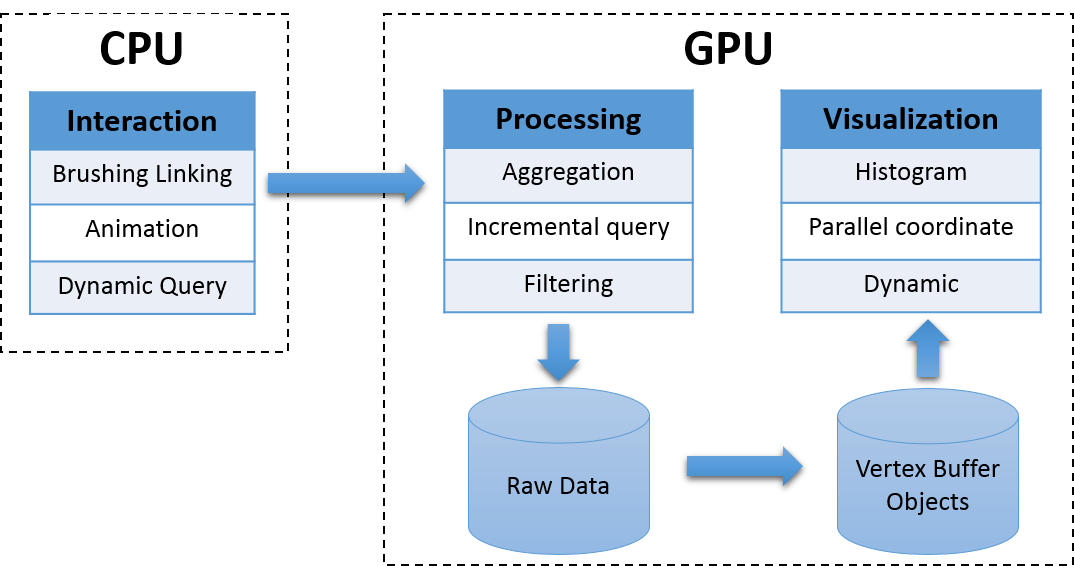
\includegraphics[width=1.0\linewidth]{pic/in-situ.png}
	\parbox[t]{1.0\columnwidth}{\relax
	}
	%
	\caption{\label{fig:architecture} The \emph{In-Situ} visualization architecture of the \emph{AVIST}.}
\end{figure}

Our in-situ visualization architecture makes best use of GPU powerful computing and rendering performance, it supports to filter and visualize items in parallel. Besides, this kind of design avoids data transformation between main memory and GPU, which is potential bottleneck for big data VA systems. 


However, the major consideration of the in-situ visualization architecture is data scalability problem, which is limited by GPU memory capability. To feed more data into the GPU memory, we propose to preprocess datasets into compressed binary format.

%There are also two major considerations in our in-situ visualization architecture. The first one is that data size is limited by GPU memory size, the second is how to deploy incremental computing idea to gain better performance.

%\subsection{Data Preprocessing}
%In our architecture, the data size is limited by GPU memory capability. To feed more data into GPU memory, we preprocess the data into compressed binary format.

For the multi-dimensional dataset, we first identify each data type in datasets. For categorical and ordinal data, we count  all possible values and map each value into a unique id. All values and their corresponding ids are stored in main memory as meta-data. While on the GPU memory, we just need to store each value's  corresponding id. Besides, based on the number of values, we store data ids in binary format of one byte, two bytes or int (e.g. if one dimension data only has less than 256 possible values, we can use one byte for representation.). For quantitative data, we simply store one \emph{int} or \emph{float} for representing each data value. We store the time data in \emph{$time\_t$} format, which occupies 8 bytes. Table \ref{preprocessing} summarizes our data preprocessing strategy.

\begin{table}[h]
	\centering
	\caption{Data preprocessing strategy}
	\label{preprocessing}
	\begin{tabular}{|c|c|c|}
		\hline
		\textbf{DataType}                                                     & \begin{tabular}[c]{@{}c@{}}\textbf{GPU memory}\\ \textbf{binary format}\end{tabular} & \begin{tabular}[c]{@{}c@{}} \textbf{Main memory} \\ \textbf{meta-data}\end{tabular}   \\ \hline
		Time                                                         & \begin{tabular}[c]{@{}c@{}}time\_t\\ 8 bytes\end{tabular}          & \begin{tabular}[c]{@{}c@{}}minimum\\  maximum\end{tabular}         \\ \hline
		Quantitative                                                 & \begin{tabular}[c]{@{}c@{}}Int or Float\\  4 bytes\end{tabular}    & \begin{tabular}[c]{@{}c@{}}minimum \\ maximum\end{tabular}         \\ \hline
		\begin{tabular}[c]{@{}c@{}}Categorial\\ Ordinal\end{tabular} & $1\sim4$ bytes                                                          & \begin{tabular}[c]{@{}c@{}}Dictionary\\ (id and data value)\end{tabular} \\ \hline
	\end{tabular}
\end{table}

A standard commercial graphics card has its memory from 4GB to 8GB. Considering a multi-dimensional dataset, most of its data attributes occupy 4 bytes, then the total data items we can handle is about 10 millions. Because data items are equal with the total transaction records multiplying its dimensions, which means that we can deal with a multi-dimensional dataset with 10 dimensions in million scale.

%We admit that this kind of design is limited by GPU memory size, and it can not handle big data scaled to terabyte. The out-of-core technique is our future, which utilizes main memory and focus on data transform between GPU memory and main memory. Better data compression techniques are the potential solutions for scaling big data in GPU.   
 
%$data items = records * dimensions$

%\subsection{Data Dependency Graph}



%// tell the in-situ concept, scientific visualization, dramel

%first identify the design require of the system architecture, then we highlight the GPU based In-Situ Architecture for big data VA system.

%data compression //raw data, meta-data preprocessing

%latency and through  rendering performance GPU In-situ 

%incremental computing Data dependency graph

%\subsection{Requirement Analysis and Design Principle}
%To real time exploratory analysis time-series and high dimensional datasets, 



\section{Visualization and Interaction in AVIST}

In AVIST, coordinated multiple views are provided for exploratory multi-dimensional data analysis. Brushing and linking, animation and dynamic queries are deployed in data views. To further improve performance and incorporate with incremental querying and animation, AVIST features a data dependency graph, which is also an instantiation of cross filtering design pattern \cite{weaver2010cross}.  


\subsection{Visualizations and Interactions}

%figure shows the design of the views. parallel 

Three data views are provided, including histogram view, parallel coordinated view and dynamic view. Figure \ref{fig:views} shows these three data views with a control panel. Other data views can also be flexible added in our architecture. For example, we add a virtual globe view for spatial data visualization in our case studies. 

\begin{figure*}[htb]
	\centering
	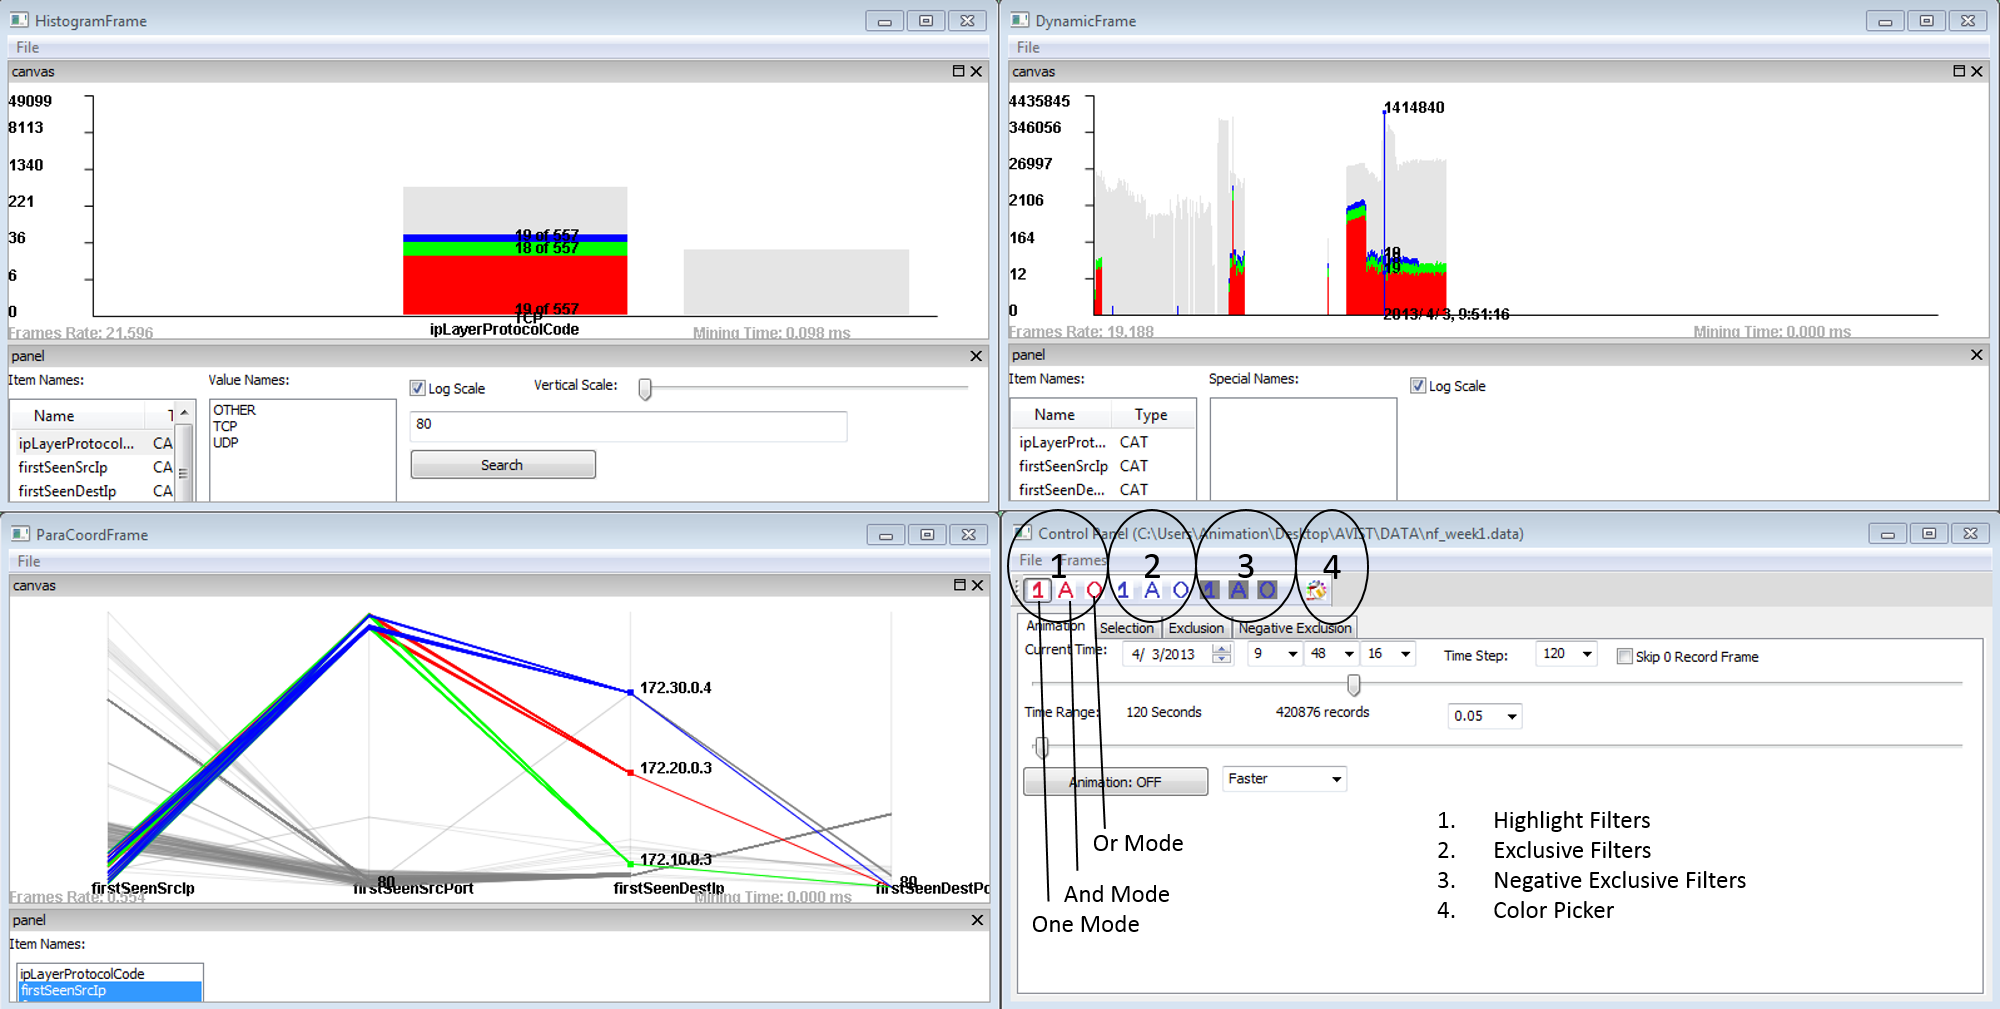
\includegraphics[width=1.0\linewidth]{pic/DataView.png}
	\parbox[t]{1.0\columnwidth}{\relax
	}
	%
	\caption{\label{fig:views}
		Three data views and control panel in AVIST system. The top left is histogram view, top right is dynamic view, bottom left is parallel coordinated view and bottom right is control panel. Each data view is separated into two parts: the canvas for rendering visual primitives and the panel for exploring different data dimensions.}
\end{figure*}  

\textbf{Histogram view} shows the data distribution in the current time window. Users can select different dimensions of datasets from a listbox to explore its aggregation information.

\textbf{Parallel coordinated view} shows the detail of each data record. Users can select multiple data dimensions for generating their custom parallel coordinate plot. The axes can be re-ordered based on users' selected order in the listbox.

\textbf{Dynamic view} is a time series stacked area chart, which shows the count changes of certain filtered events over a period of time. When user change data filters, the dynamic view clears previous visual primitives and re-draw everything again. 

\textbf{Control panel} provides the user interactions related with animation. By playing the animation of the data changes in certain pace, the hidden temporal patterns can be revealed. The animation control supports automatic forward playback, interactively dragging of the time line bar, and interactive change of animation speed. With the change of the current time and time range, user can define a time window in which the information will be analyzed and visualization on these correlated views. By combining automated animation with these correlated views, AVIST provides the temporal changes in the datasets, therefore to discover interesting temporal patterns for further analysis.

Besides the time window for filtering data, AVIST features the combined data filters. Three different filters are implemented: 1) highlight filters, which make the user selected values stand out of the rest data with different colors,  2) exclusive filters to remove non-interesting data from the data views and 3) negative exclusive filters, which are the exact opposite of exclusive filters, to remove all data while keeping user interesting items. Each kind of data filters have three  modes: 1) \emph{one mode} , which allows only one filter value in current filter, 2) \emph{and mode}  to combine several filters together as a complex filter, which emphasizes that data records need satisfy all requirements for visualization and 3) \emph{or mode}, which means that data records just need meet one of the filter requirements. 



Based on these three basic filters with their three modes, user can nest them to generate complex data filters, which help users to drill down each piece of data record from big overview visualization. These filters with the brushing and linking interaction technique can quickly help users to explore datasets. In Figure \ref{fig:views}, users select  highlight filters with \emph{or mode}, and then brush their selected colors in \textit{firstSeenDespIp} axis of parallel coordinated view to identify port scan behavior, which starts from three machines. The histogram view shows the distributions of \textit{ipLayerProtocol}, indicating the port scan behavior happens only in TCP flows. And the dynamic view shows that the port scan is a periodically behavior in the network. 

%for visual analysis large cyber security datasets, users can directly apply exclusive filter on port 80 to remove related network records to clear the visualization. After it, all three data views are immediately updated, and potential visual patterns may appear.

\subsection{Data Dependency Graph}

% consider the cross filter design pattern 
We employ the cross filtering design pattern \cite{weaver2010cross} in our GPU based in-situ visualization architecture, which results in a data dependency graph for organizing the data flow in the GPU.

Figure \ref{fig:datagraph} shows our data dependency graph, which is separated into three parts. The first part of top level graph shows the user interactions in CPU side. Users can manipulate four filters based on their interactions: \emph{time windows}, \emph{exclusive filter}, \emph{negative exclusive filter} and \emph{highlight filter}. All filters are passed into GPU side for data processing. The middle part of the graph is the GPU data parallel processing. The raw data is filtered by \emph{time windows} first, then both \emph{exclusive filter} and \emph{negative exclusive filter} are applied to remove users' uninteresting or unnecessary data items. At last, \emph{highlight filter} is deployed to generate highlight dataset,  then followed two steps to transform the original data items into visual primitives in each data view. The first one is to generate geometry data, which are mainly about lines positions and widths, the size of rectangle and so on. The second step is about rendering data, and it applies projection matrix, viewport and other visual parameters to geometry data. At last, all rendering data are passed into GPU VBOs. This kind of design makes that all data views share the raw data, filtered data and highlight filtered data, while each data view has its own geometry and rendering data. The last part in this graph is GPU rendering, which transforms all visual primitives into pixel colors.  

 \begin{figure}[htb]
 	\centering
 	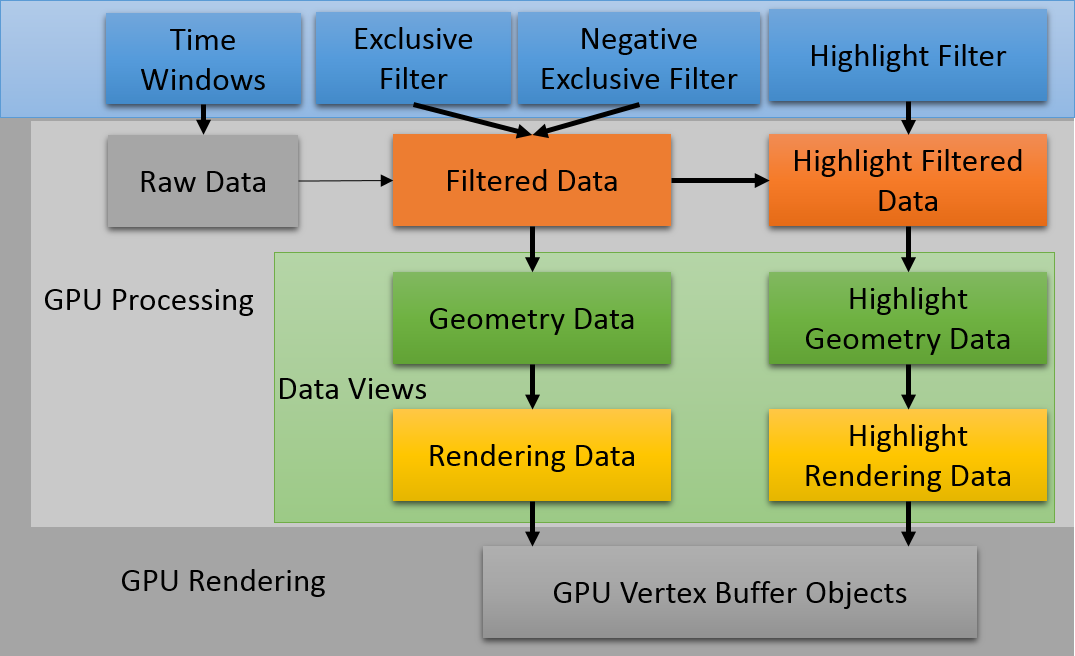
\includegraphics[width=1.0\linewidth]{pic/graph.png}
 	\parbox[t]{1.0\columnwidth}{\relax
 	}
 	%
 	\caption{\label{fig:datagraph} The data dependency graph of AVIST system.}
 \end{figure} 
 
 
Our data dependency graph has several advantages. First, it follows the cross filtering design pattern \cite{weaver2010cross}, and three filters with three modes supports the drill down query of multi-dimensional datasets. Users interactions trigger the data flows to update the visualizations. Second, all data processing and visual rendering can fully utilize GPU resources to achieve best performance. Third,  incremental computing can be applied. When users play animation, frame-to-frame coherence can be exploited. In such cases, only incremental data need to be considered. Besides, user interactions also follow incremental format for dill-down queries. If user perform \emph{or} operator of highlight filters, previous highlighting visual primitives do not need to re-computer again. When performing \emph{and} operator, incremental computing is only applied to previous highlight data to trigger the right column of data graph, while all other data are still the same.
 
%one page
%// and or not similar with SQL  ad hoc visual query
%//multiple coordinate views space 
%//animation 	time

\section{Implementation}
In this section, we first describe our GPU based solution for implementing AVIST system, then we provide detailed performance analysis of our system.

\subsection{Filtering on the GPU}
The implementation of time windows filter is straightforward, and we apply binary search of the raw data to obtain the start and end records within the time window (The raw data is stored chronologically). We generate a boolean vector, and examine each records by the exclusive filter and negative exclusive filter. Then we compact the boolean vector and 
\subsection{Data View on the GPU}
The dynamic view and histogram view is simple, and we focus on the parallel coordinate generation on the GPU.
The input data is the filtered or highlighted filtered data, and the output is the edge list and node position.
We use shader to generate the stack view and quad.
\subsection{Performance Analysis}
The AVIST system is written in C++ and CUDA 5.5. The visualization codes are based on OpenGL and GLSL. The interface controls are coded using wxWidgets.

We test the performance of AVIST system on a desktop computer, running Windows 7 Enterprise with Service Pack 1, which is equipped with an Intel i7 processor and an NVIDIA GeForce GTX 680 graphics card with 4GB memory. And we use the network traffic dataset from case study one as the benchmark to profile AVIST system.  



Based on our data dependency graph, we character the AVIST system in two stages. The first stage is about filtered data generation. This stage is shared by all data views. The second stage is each data view visual primitives generation, and their performance are independent with each other. Figure \ref{fig:performance} shows the performance in scatter plots. We see that the performance has a linear relationship with the queried data records except the dynamic view. Actually, the aggregated information in dynamic view can be easily derived by filtered dataset. The performance of parallel coordinated view is the bottleneck in AVIST system, because it generates a number of visual primitives to match each data record. If the number of queried records exceeds 600,000, AVIST can not afford real time animation and interaction due to the hardware computation limitation. This also suggests that user should filter more data in current time window or shrink his time window size to drill-down query the data details.

\begin{figure}[htb]
	\centering
	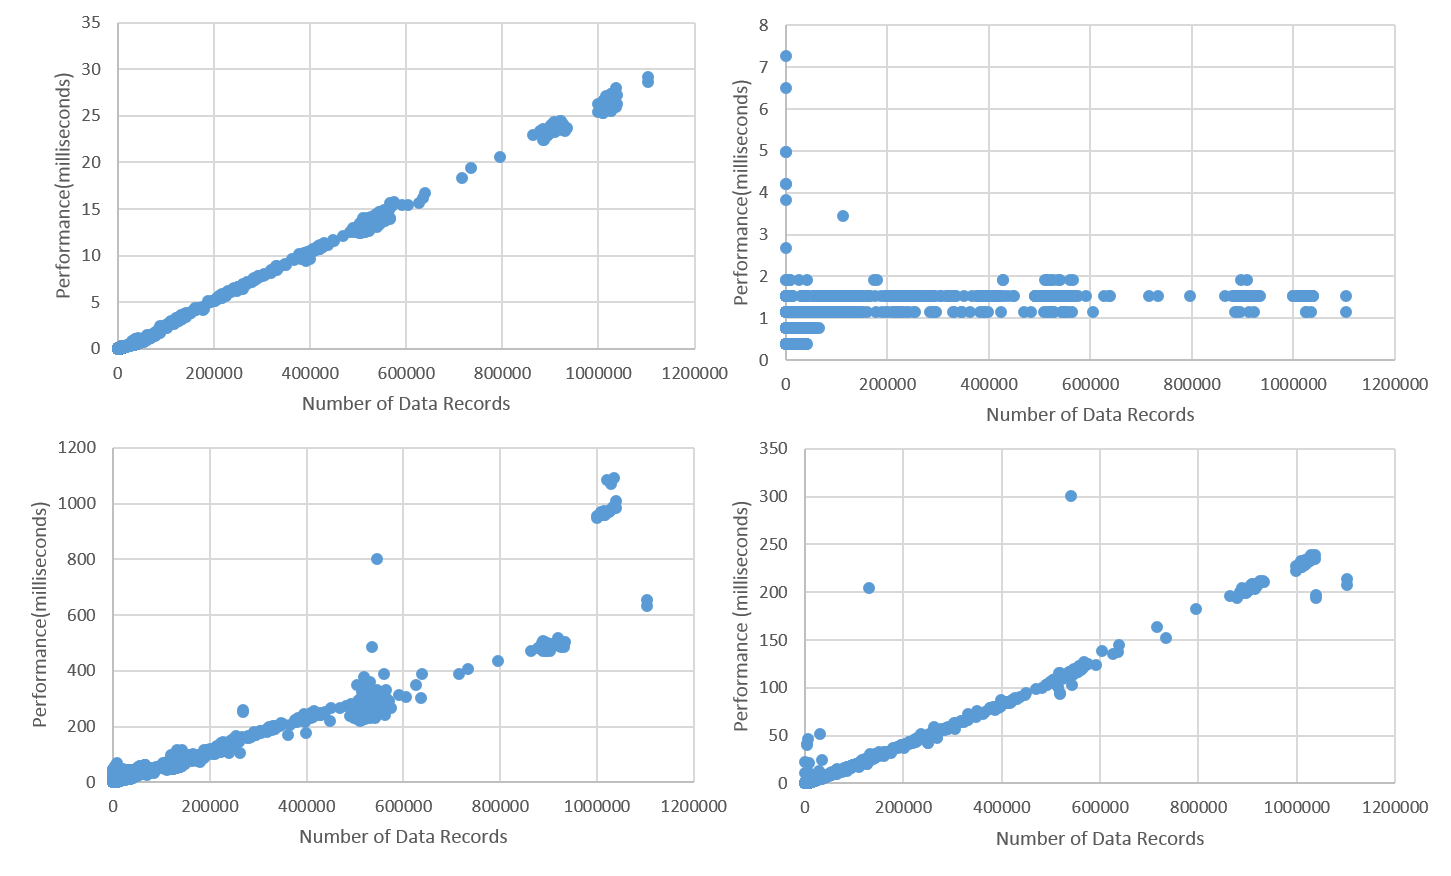
\includegraphics[width=1.0\linewidth]{pic/performance.png}
	\parbox[t]{1.0\columnwidth}{\relax
	}
	%
	\caption{\label{fig:performance}
		The performance of AVIST system. These scatter plots show the relationship between number of queried data records and the performance (milliseconds). From the top left to the bottom right are the performances of histogram view, dynamic view, parallel coordinated view and the filtered data.  }
\end{figure}

\section{User Cases}
Below we describe two examples AVIST explorations of large volume of time series and multidimensional datasets. We show how data patterns are revealed by animation and drilling down queries and show how AVIST system is applied for large spatial-temporal data analysis.

\subsection{Network Flow Analysis} %Cyber Security Analysis

\begin{figure*}[htb]
	\centering
	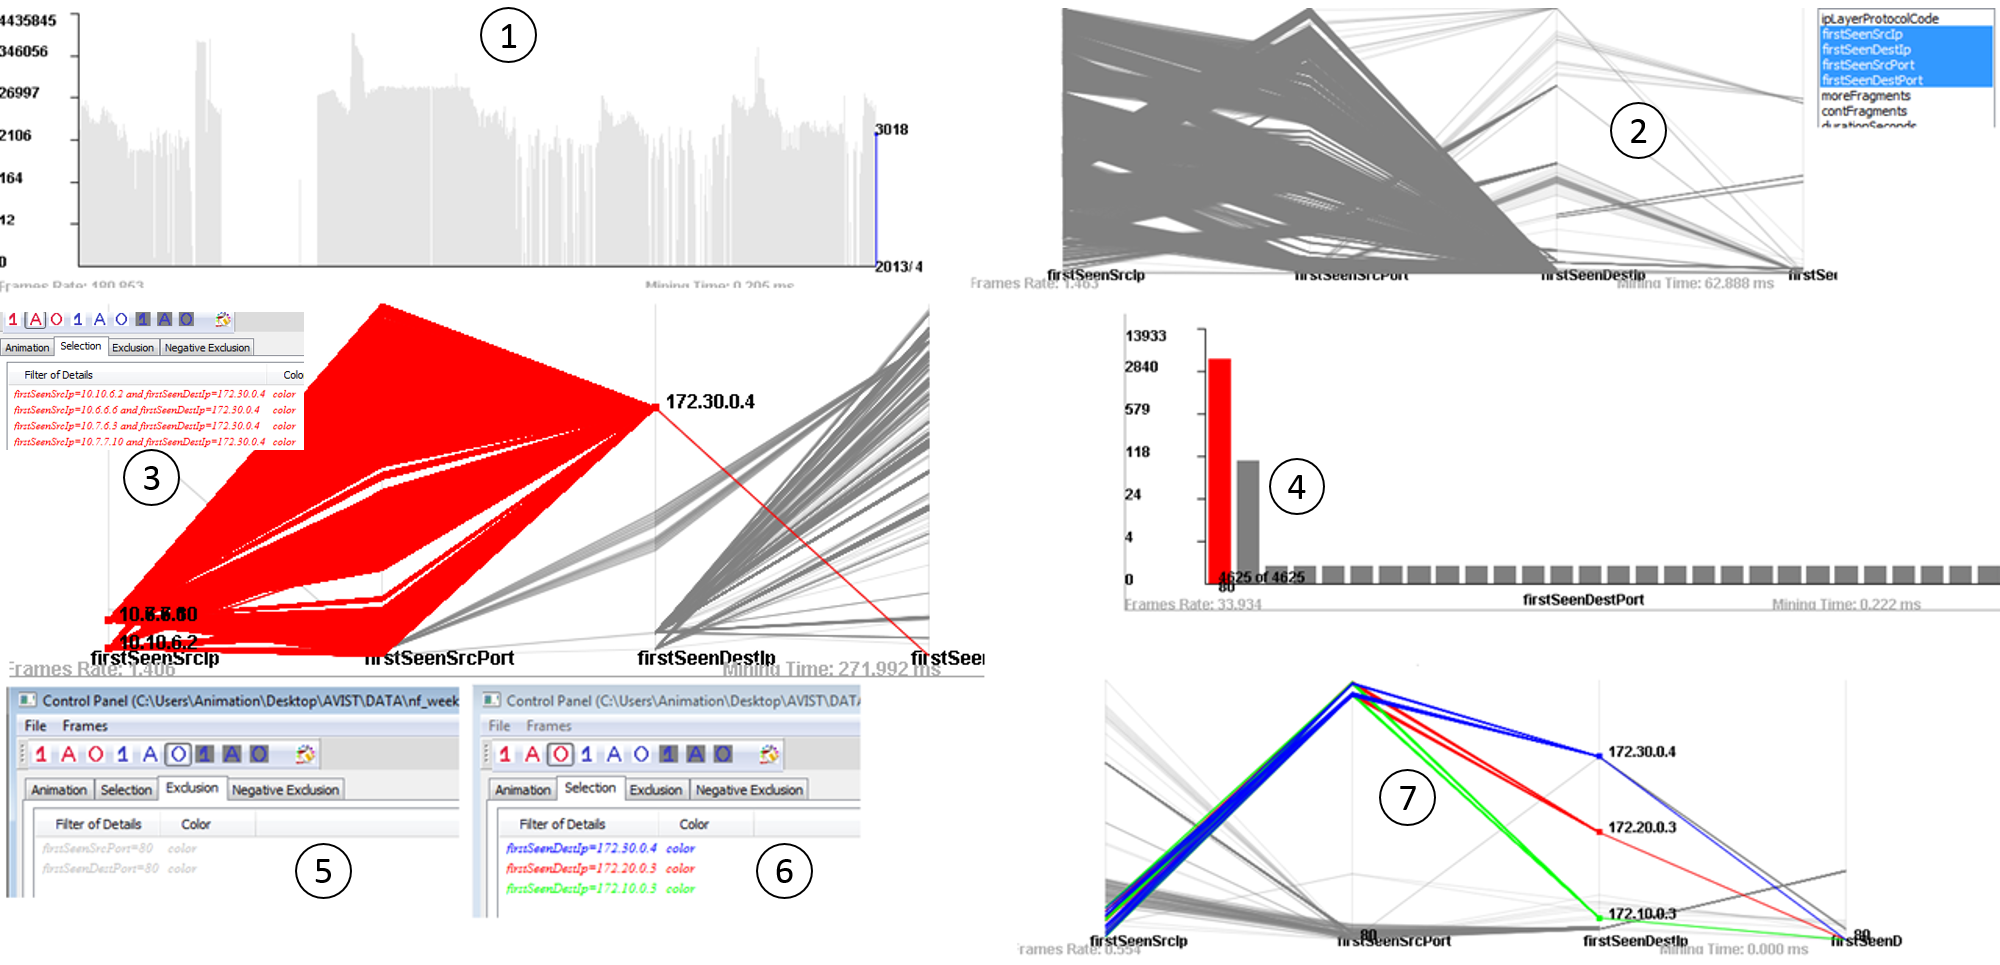
\includegraphics[width=1.0\linewidth]{pic/network2.png}
	\parbox[t]{1.0\columnwidth}{\relax
	}
	%
	\caption{\label{fig:network}
		This figure shows a usage scenario how AVIST system helps analysts to visual explore the large network logs. 
		Seven steps are presented in this figure, and Section 7.1 gives more detailed discussions for each step. }
\end{figure*}

Exploratory visual analysis network logs is critical for detecting potential cyber threats and network intrusions. VAST 2013 Mini Challenge 3, which targets the analysis of Big Marketing company's network, provides big network traffic and a variety of logs\footnote{http://vacommunity.org/VAST+Challenge+2013}. Among all the datasets,  the biggest one is about week one network flow, which includes 46,138,310 records with 16 dimensions, so as the total data items is about 738,212,960. 

Analysts first preprocess original dataset, and obtain the compressed binary data with 1.8GB. Then analysts load the data into AVIST system to explore the network traffic and to identify the potential threats. Figure \ref{fig:network} shows one usage scenario to demonstrate how analysts find potential network security threats and detect temporal patterns based on AVIST system. 

First of all, analysts specify animation speed and time window size (120 seconds in this example) to play animation. The overview of network traffic is visualized in dynamic view, shown in subgraph 1. Analysts then identify an unusual behavior that there is no any network flow from 4-2-2013 9:40 am to 4-3-2013 3:26 am. To investigate the details, analysts generate the parallel coordinate view in subgraph 2 by choosing data dimensions in order of \emph{firstSeenSrcIp}, \emph{firstSeenSrcPort}, \emph{firstSeenDestIp} and \emph{firstSeenDestPort}. Analysts then play animation again and discover an interesting visual pattern. Analysts character this pattern by highlight related data records. In subgraph 3, they learn that the destination ip 172.30.0.4 was accessed by four source IPs 10.10.6.2, 10.6.6.6, 10.7.6.5, 10.7.7.10 from their all available ports during 4-2-2013 5:20 am. However, analysts find that the parallel coordinate view are always over-cluttered.  Subgraph 4 shows the network traffic distribution based on \emph{firstSeenDestPort}, and analysts realize that most of the network records are related with port 80. They first assume that these records may be normal and they want to remove these data records to see buried patterns, so they apply exclusive filters to remove these network logs visualization in subgraph 5. Then they discover a port scan behavior from parallel coordinate view in subgraph 7, and they character this pattern by applying different colors in each highlight filter, shown in subgraph 6.  The whole picture of port scan behavior is shown in Figure \ref{fig:views}. Analysts play and play back animation, and identify that the port scan only happens in TCP flow and it may be a periodical behavior. All of those information can guide analysts next visual query interaction to infer more.


%Dynamic view provides the overview of one week's network flow in subgraph 1. Analysts find there is no any network data from 4-2-2013 9:40 am to 4-3-2013 3:26 am, which is unusual, and they suspect that the whole network had been crushed. To investigate the details, analysts choose source ip and port, destination ip and port to generate parallel coordinate view in subgraph 2. Analysts then play animation again and identify an interesting pattern in subgraph 3. Analysts confirm this behavior details by highlighting related data records, and they find that destination ip 172.30.0.4 was trying to scan three ips during 4-2-2013 5:20 am.  However, the parallel coordinate view are over-cluttered most of the time. Based on histogram view in subgraph 4, analyst find most of network flow are related with port 80. They infer that these network flow may be normal behavior, which may just access company's homepage. Analysts apply exclusive filters to remove these network logs in subgraph 5. 

%Subgraph 6 shows that analysts apply different colors in highlight filers to identify the port scan behavior in parallel coordinate view of subgraph 7.

%they play animation again to identify the behavior distribution in histogram view and dynamic view. They find that the port scan may be a periodical behavior and it happens in TCP transactions. These information may infer analysts next interaction to query more.

%Figure \ref{fig:views} shows the whole picture of  port scan behavior. After analysts highlight three suspicious ips, 

This scenario shows that AVIST system can facilitate analysts incremental and dirll-down query for exploratory analysis the big network traffic. The combined data filters can help analysts easily to remove visual clutter and to character abnormal patterns. By playing animation, analysts can identify temporal behaviors to infer more. 
 
%From this scenario, analysts can real time exploratory visual analysis the whole dataset by animation and drill-down queries. They could quickly make sense of big network logs, to iteratively refine their findings to each data records from the overview. 
%//short time visual explore from the overview to detail. and 

 



\subsection{International Trade Analysis}
Making sense of international trade is important for government and police makers. With the world economic growth, world trade transactions become large and complex. In this case study, we obtain big international trade transactions from PIERS Global Intelligence Solutions\footnote{https://www.piers.com/}, a private company that provides portfolio analysis for U.S. waterborne trade activity in the world. The dataset is about 2013 US waterborne imports from other countries, with 10,735,092 records and 10 dimensions, so total data items is 107,350,920. Among 10 dimensions, each data records features the US port code and foreign port code, which illustrates the geospatial information in each record.

We first preprocess the original dataset, and obtain the compressed data with 266MB. To facilitate analysts to explore the geospatial data, we incorporate a virtual globe view in AVIST, and its implementation follows the data dependency graph design. In this case study, we emphasis the hypothesis generation and verification.
And figure \ref{fig:architecture} shows a usage scenario how analysts explore the big spatial-temporal international trades to gain insights.

\begin{figure*}[htb]
	\centering
	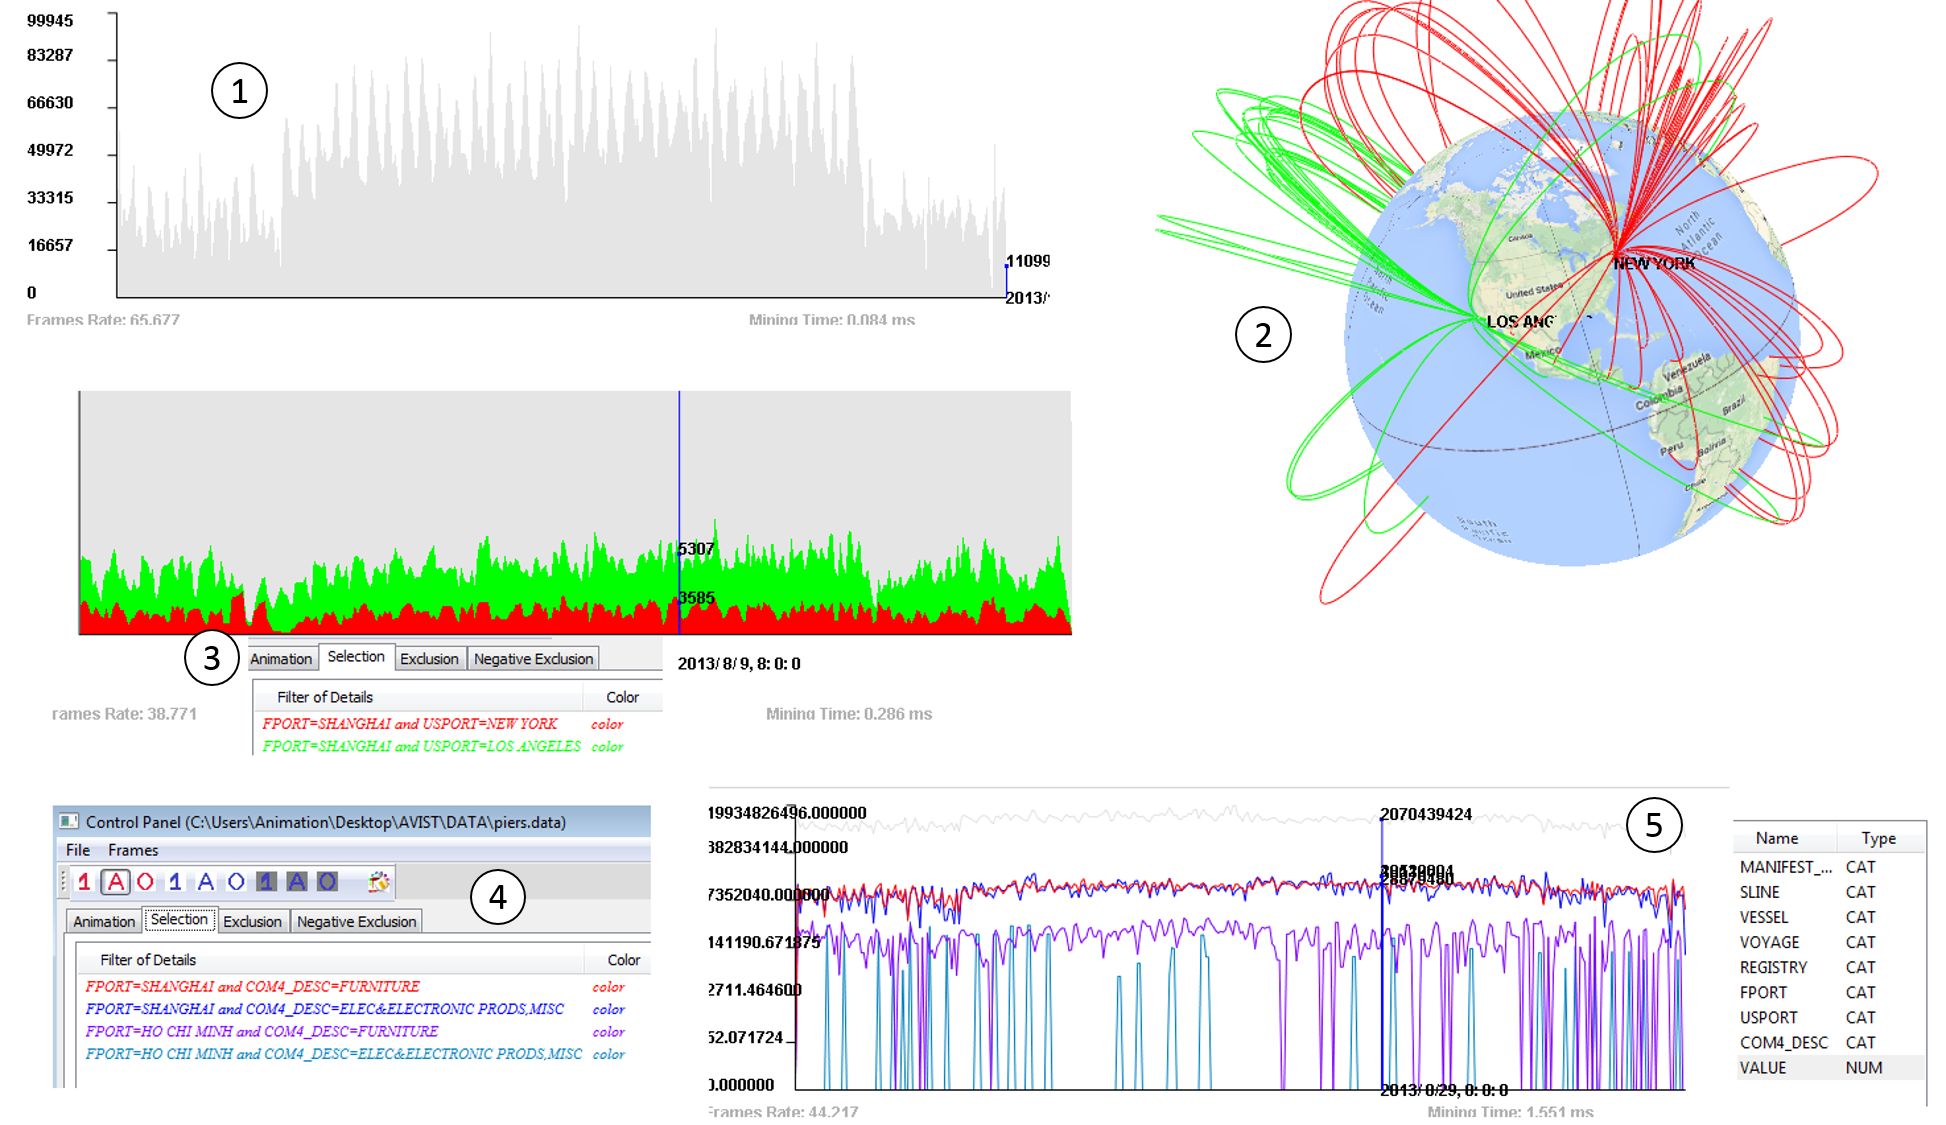
\includegraphics[width=1.0\linewidth]{pic/worldtrade2.png}
	\parbox[t]{1.0\columnwidth}{\relax
	}
	%
	\caption{\label{fig:network}
		This figure shows the usage scenario that analysts use AVIST system to visual explore big international trade transactions. The detailed discussions are presented in Section 7.2.}
\end{figure*}

Firstly, analysts specify the time window (86400 seconds or one day) before playing animation. The dynamic view shows the overview of the world trades in subgraph 1, which reveals that the international trades are clearly separated into four quarters. The second and third quarters has more transactions than others. Analysts hypothesize that the international trades may also have some spatial patterns. They highlight two US ports: Los Angeles (LA) and New York (NY). They suppose that LA has more trades with pacific countries while NY is more related with Western European because the waterborne trade may be more sensitive with geolocations. Subgraph 2 shows one snapshot of records with this two ports in virtual globe view. To verify it, analysts create two highlight filters, focusing the records from ShangHai (SH) to LA and NY. They play animation and generate the dynamic view in subgraph 3. They find that the trades from SH to LA is roughly twice of trades to NY, which supports  their hypothesis. The international trades also character country's economy. Analyst generate four filters to compare the economy of China and Vietnam. They choose ShangHai port and Ho Chi Minh port for representing these two countries, and target the trades related with furniture and electronics, as shown in subgraph 4. They are more interested in the money value rather than the number of trades records, so they click the value in the listbox and play animation. Subgraph 5 is the dynamic view with four highlighted line charts, which shows that two kinds of trades are more balanced in China economy and Vietnam more relies on furniture in its exports. 

%This scenario shows that AVIST system can help analysts quickly generate and verify their hypothesis based on exploratory analysis.         
   




%Firstly, analysts can specify animation speed and time window size (120 seconds in this example) to play animation. Dynamic view provides the overview of one week's network flow in subgraph 1. Analysts find there is no any network data during 4-2-2013 9:40 am to 4-3-2013 3:26 am, which  indicates that the whole network had been crushed. To investigate the details, analysts choose source ip and port, destination ip and port to generate parallel coordinate view in subgraph 2. Analysts then play animation again and find unusual pattern in subgraph 3. Analysts identify this pattern's details using highlight filters, and they find that machine 172.30.0.4 was trying to scan three machine during 4-2-2013 5:20 am.  However, visualization of parallel coordinate view are always over-cluttered. In histogram view of subgraph 4, analyst find most of network flow are from port 80. These network flow may be normal to access company's webpage. Analysts apply exclusive filters to remove the network logs, which had access 80 port in subgraph 5. Subgraph 6 shows that analysts use different color to highlight source ips to reveal the port scan behavior in subgraph 7. Figure \ref{fig:views} shows the whole picture of  port scan behavior. After analysts highlight three suspicious ips, they play animation again to identify the behavior distribution in histogram view and dynamic view. They find that the port scan may be a periodical behavior and it happens in TCP transactions. These information may infer analysts next interaction to query more.

%\\the data, and analysis want to compare and geolocation information 




%mining golden in big data

%is filtered data generation based on time window filter. The second is each data view's geometry data, then is rendering data, and the last one is the GPU rendering performance. 
 
%The performance of AVIST system is related with a number of factors: the number of data views, the visual primitive in each data view, time window size, and the data velocity. Based on our data dependency graph design, each view has its own data processing stage for generating their visual primitives, which means the performance of each data views is independent. In this section, we character the performance of AVIST system for the three data views. Because the time window size can change the data velocity: larger time window size indicates more data item, so we analyze the relationship of each data performance with number of data items.   
%Firstly, analysts can specify animation speed and time window size (120 seconds in this example) to play animation. Dynamic view provides the overview of one week's network flow in subgraph 1. Analysts find there is no any network data during 4-2-2013 9:40 am to 4-3-2013 3:26 am, which  indicates that the whole network had been crushed. To investigate the details, analysts choose source ip and port, destination ip and port to generate parallel coordinate view in subgraph 2. Analysts then play animation again and find unusual pattern in subgraph 3. Analysts identify this pattern's details using highlight filters, and they find that machine 172.30.0.4 was trying to scan three machine during 4-2-2013 5:20 am.  However, visualization of parallel coordinate view are always over-cluttered. In histogram view of subgraph 4, analyst find most of network flow are from port 80. These network flow may be normal to access company's webpage. Analysts apply exclusive filters to remove the network logs, which had access 80 port in subgraph 5. Subgraph 6 shows that analysts use different color to highlight source ips to reveal the port scan behavior in subgraph 7. Figure \ref{fig:views} shows the whole picture of  port scan behavior. After analysts highlight three suspicious ips, they play animation again to identify the behavior distribution in histogram view and dynamic view. They find that the port scan may be a periodical behavior and it happens in TCP transactions. These information may infer analysts next interaction to query more.

\section{Discussion And Limitations}

To facilitate exploratory visual analysis big data, we argue VA system should support user's drill down query. Based on this guideline, we have summarized previous techniques considering both system performance and user interactions. 
We emphasize the \emph{in-situ} concept in visual analytics field to support real-time querying big data, and we present a GPU based in-situ visualization architecture, to utilize powerful GPU computing and rendering resources to achieve this. A number of human interaction techniques are also considered to help user to quickly explore big data. And we incorporate these techniques into a data dependency graph based on the GPU in-situ architecture design. As a proof of concept, we present AVIST system and show two cases to demonstrate our ideas.

There are, however, some limitations in our current system. We design to store all the raw data in the GPU memory, which limits the data size by the GPU memory capability. Even we suggest to compress the data into its binary format, the current GPU memory could only support no more than 10 million data items. Our design fails to handle big data, when the number of data scales to billion and trillion. Besides large volume, big data also features in large variety and velocity \cite{schroeck2012analytics}. However, our current design has no good solution to cover these two areas. For example, AVIST cannot handle more than 600,000 data items at once to afford real time performance.

AVIST system only targets for exploratory visual analysis of big time-series and multidimensional datasets. By slicing such big data from time dimension and filtering from other dimensions, AVIST supports the drill-down query. In real world, big data are much more complex. FaceBook has billions of friends relationships and Amazon has tons of users, reviews, goods. Our current design and implementation cannot scale to these datasets.   

%The main contribution of this paper is the \emph{in-situ}
%We borrow the \emph{in-situ} concept from scientific visualization filed, and present a GPU based in-situ visualization architecture, which features the computing and rendering running simultaneously to reduce I/O costs. To utilize powerful GPU resources,       
 
%In this paper, we presented AVIST system for exploratory visual analysis big data. 
%p1: our contributions
%p2:  cirtical previous design
%p3: continue say our contribution
%p4: limiattions
 


\section{Conclusions And Future Work}
In this paper, we highlight the \emph{in-situ} processing and visualizing in visual analysis field to real time explore big time-series and multidimensional data. We propose a GPU based in-situ visualization architecture to fully utilize the GPU computing and rendering capability. We implement the AVIST system as a proof of concept, and carefully design a data dependency graph in the system to incorporate several human interaction techniques. We have shown the effectiveness of AVIST system through two usage cases. Finally, we have shown the performance analysis of our system and discussed limitations.  

There are several directions to continue our research. First, we want to investigate new data lossless compression techniques to feed more data on the GPU memory. Second, more data views and functionalities need be implemented to support better exploratory visual analysis. Finally, comprehensive user studies need be conducted, especially compared with the existing VA softwares such as \emph{Tableau}\cite{tab}, \emph{Spotfire}\cite{spotfire}, \emph{QlikView}\cite{qlikview} and so on to investigate the future of VA systems.  
%We presented AVIST system - a GPU based animation visualization toolkit for exploratory visual analysis large time-series and multidimensional dataset.

%p1: contribution what we did, and why it is useful, point 1, point 2, combined together
%p2: future work

%Firstly, analysts can specify animation speed and time window size (120 seconds in this example) to play animation. Dynamic view provides the overview of one week's network flow in subgraph 1. Analysts find there is no any network data during 4-2-2013 9:40 am to 4-3-2013 3:26 am, which  indicates that the whole network had been crushed. To investigate the details, analysts choose source ip and port, destination ip and port to generate parallel coordinate view in subgraph 2. Analysts then play animation again and find unusual pattern in subgraph 3. Analysts identify this pattern's details using highlight filters, and they find that machine 172.30.0.4 was trying to scan three machine during 4-2-2013 5:20 am.  However, visualization of parallel coordinate view are always over-cluttered. In histogram view of subgraph 4, analyst find most of network flow are from port 80. These network flow may be normal to access company's webpage. Analysts apply exclusive filters to remove the network logs, which had access 80 port in subgraph 5. Subgraph 6 shows that analysts use different color to highlight source ips to reveal the port scan behavior in subgraph 7. Figure \ref{fig:views} shows the whole picture of  port scan behavior. After analysts highlight three suspicious ips, they play animation again to identify the behavior distribution in histogram view and dynamic view. They find that the port scan may be a periodical behavior and it happens in TCP transactions. These information may infer analysts next interaction to query more.


\bibliographystyle{abbrv}
%%use following if all content of bibtex file should be shown
%\nocite{*}
\bibliography{template}
\end{document}

